
\let\negmedspace\undefined
\let\negthickspace\undefined
\documentclass[journal,12pt,twocolumn]{IEEEtran}
%\documentclass[conference]{IEEEtran}
%\IEEEoverridecommandlockouts
% The preceding line is only needed to identify funding in the first footnote. If that is unneeded, please comment it out.
\usepackage{svg}
\usepackage{tikz}
\usepackage{cite}
\usepackage{amsmath,amssymb,amsfonts,amsthm}
\usepackage{algorithmic}
\usepackage{float}
\usepackage{graphicx}
\usepackage{subcaption}
\usepackage{xcolor}
\usepackage{txfonts}
\usepackage{listings}
\usepackage{enumitem}
\usepackage{mathtools}
\usepackage{gensymb}
\usepackage[breaklinks=true]{hyperref}
\usepackage{tkz-euclide} % loads  TikZ and tkz-base
\usepackage{listings}
\usetikzlibrary{positioning}
%
%\usepackage{setspace}
%\usepackage{gensymb}
%\doublespacing
%\singlespacing

%\usepackage{graphicx}
%\usepackage{amssymb}
%\usepackage{relsize}
%\usepackage[cmex10]{amsmath}
%\usepackage{amsthm}
%\interdisplaylinepenalty=2500
%\savesymbol{iint}
%\usepackage{txfonts}
%\restoresymbol{TXF}{iint}
%\usepackage{wasysym}
%\usepackage{amsthm}
%\usepackage{iithtlc}
%\usepackage{mathrsfs}
%\usepackage{txfonts}
%\usepackage{stfloats}
%\usepackage{bm}
%\usepackage{cite}
%\usepackage{cases}
%\usepackage{subfig}
%\usepackage{xtab}
%\usepackage{longtable}
%\usepackage{multirow}
%\usepackage{algorithm}
%\usepackage{algpseudocode}
%\usepackage{enumitem}
%\usepackage{mathtools}
%\usepackage{tikz}
%\usepackage{circuitikz}
%\usepackage{verbatim}
%\usepackage{tfrupee}
%\usepackage{stmaryrd}
%\usetkzobj{all}
%    \usepackage{color}                                            %%
%    \usepackage{array}                                            %%
%    \usepackage{longtable}                                        %%
%    \usepackage{calc}                                             %%
%    \usepackage{multirow}                                         %%
%    \usepackage{hhline}                                           %%
%    \usepackage{ifthen}                                           %%
  %optionally (for landscape tables embedded in another document): %%
%    \usepackage{lscape}     
%\usepackage{multicol}
%\usepackage{chngcntr}
%\usepackage{enumerate}

%\usepackage{wasysym}
%\newcounter{MYtempeqncnt}
\DeclareMathOperator*{\Res}{Res}
%\renewcommand{\baselinestretch}{2}
\renewcommand\thesection{\arabic{section}}
\renewcommand\thesubsection{\thesection.\arabic{subsection}}
\renewcommand\thesubsubsection{\thesubsection.\arabic{subsubsection}}

\renewcommand\thesectiondis{\arabic{section}}
\renewcommand\thesubsectiondis{\thesectiondis.\arabic{subsection}}
\renewcommand\thesubsubsectiondis{\thesubsectiondis.\arabic{subsubsection}}

% correct bad hyphenation here
\hyphenation{op-tical net-works semi-conduc-tor}
\def\inputGnumericTable{}                                 %%
\newcommand{\permcomb}[4][0mu]{{{}^{#3}\mkern#1#2_{#4}}}
\newcommand{\comb}[1][-1mu]{\permcomb[#1]{C}}
\lstset{
%language=C,
frame=single, 
breaklines=true,
columns=fullflexible
}
%\lstset{
%language=tex,
%frame=single, 
%breaklines=true
%}

\begin{document}
%


\newtheorem{theorem}{Theorem}[section]
\newtheorem{problem}{Problem}
\newtheorem{proposition}{Proposition}[section]
\newtheorem{lemma}{Lemma}[section]
\newtheorem{corollary}[theorem]{Corollary}
\newtheorem{example}{Example}[section]
\newtheorem{definition}[problem]{Definition}
%\newtheorem{thm}{Theorem}[section] 
%\newtheorem{defn}[thm]{Definition}
%\newtheorem{algorithm}{Algorithm}[section]
%\newtheorem{cor}{Corollary}
\newcommand{\BEQA}{\begin{eqnarray}}
		\newcommand{\EEQA}{\end{eqnarray}}
\newcommand{\define}{\stackrel{\triangle}{=}}

\bibliographystyle{IEEEtran}
%\bibliographystyle{ieeetr}


\providecommand{\mbf}{\mathbf}
\providecommand{\pr}[1]{\ensuremath{\Pr\left(#1\right)}}
\providecommand{\qfunc}[1]{\ensuremath{Q\left(#1\right)}}
\providecommand{\sbrak}[1]{\ensuremath{{}\left[#1\right]}}
\providecommand{\lsbrak}[1]{\ensuremath{{}\left[#1\right.}}
\providecommand{\rsbrak}[1]{\ensuremath{{}\left.#1\right]}}
\providecommand{\brak}[1]{\ensuremath{\left(#1\right)}}
\providecommand{\lbrak}[1]{\ensuremath{\left(#1\right.}}
\providecommand{\rbrak}[1]{\ensuremath{\left.#1\right)}}
\providecommand{\cbrak}[1]{\ensuremath{\left\{#1\right\}}}
\providecommand{\lcbrak}[1]{\ensuremath{\left\{#1\right.}}
\providecommand{\rcbrak}[1]{\ensuremath{\left.#1\right\}}}
\theoremstyle{remark}
\newtheorem{rem}{Remark}
\newcommand{\sgn}{\mathop{\mathrm{sgn}}}
\providecommand{\abs}[1]{\(left\)vert#1\(right\)vert}
\providecommand{\res}[1]{\Res\displaylimits_{#1}}
\providecommand{\norm}[1]{\(left\)lVert#1\(right\)rVert}
%\providecommand{\norm}[1]{\lVert#1\rVert}
\providecommand{\mtx}[1]{\mathbf{#1}}
\providecommand{\mean}[1]{E\(left\)[ #1 \(right\)]}
\providecommand{\fourier}{\overset{\mathcal{F}}{ \rightleftharpoons}}
%\providecommand{\hilbert}{\overset{\mathcal{H}}{ \rightleftharpoons}}
\providecommand{\system}{\overset{\mathcal{H}}{ \longleftrightarrow}}
%\newcommand{\solution}[2]{\textbf{Solution:}{#1}}
\newcommand{\solution}{\noindent \textbf{Solution: }}
\newcommand{\cosec}{\,\text{cosec}\,}
\providecommand{\dec}[2]{\ensuremath{\overset{#1}{\underset{#2}{\gtrless}}}}
\newcommand{\myvec}[1]{\ensuremath{\begin{pmatrix}#1\end{pmatrix}}}
\newcommand{\mydet}[1]{\ensuremath{\begin{vmatrix}#1\end{vmatrix}}}

\let\vec\mathbf


\vspace{3cm}

\title{
	%	\logo{
	Assignment:- 4
 
	\Large AI1110: Probability and Random Variables
 
	\Large Indian Institute of Technology, Hyderabad
	%	}
}
\author{
	CS22BTECH11001
	
	Aayush Adlakha
 
	29 April, 2023
	% <-this % stops a space
}






\maketitle

\newpage


\bigskip
\renewcommand{\thefigure}{\theenumi}
\renewcommand{\thetable}{\theenumi}
\textbf{12.13.6.4}
Suppose that 90 \% of people are right handed. What is the probability that
at most 6 of a random sample of 10 people are right-
handed.

\textbf{Solution.}
Let $X$ be a Binomial random Variable.
\begin{align}
    X&=Bin(n,p)\\
    &=Bin(10,0.9)
\end{align}
The mean $\mu$ of $X$,
\begin{align}
    \mu &= n\times p\\
    &= 9
\end{align}
The Variance $\sigma^2$ of $X$,
\begin{align}
    \sigma^2 &= n\times p\times (1-p)\\
    &= 0.9
\end{align}
Let,
\begin{align}
    Z&=\frac{X-\mu}{\sigma}
\end{align}
Now, $Z$ is a random variable with $\mu=0$ and $\sigma^2=1$.

We can calculate the distribution of $Z$ by assuming it be a set of discrete points on the Normal-Distribution.

Note:-The CDF of Z will converge to the normal distribution for large values of $n$.

[Proof on next page]

The Normal-Distribution,
\begin{align}
    f(x) = \frac{1}{\sqrt{2\pi}}\times e^{-\frac{x^2}{2}}
\end{align}
The Q-function from the Normal-Distribution
\begin{align}
    Q(x) &=\pr{Z>x}\\
    \pr{Z>x}&=\int_{x}^{\infty} \frac{1}{\sqrt{2\pi}}\times e^{-\frac{t^2}{2}} \,dt\\\
    Q(x)&=\int_{x}^{\infty} \frac{1}{\sqrt{2\pi}}\times e^{-\frac{t^2}{2}} \,dt\
\end{align}

\begin{align}
    X &< 6.5\\
    \therefore Z &< \frac{6.5-\mu}{\sigma}\\
    Z&<-2.63
\end{align}
Note:- The additional 0.5 correction term is present.
We want
\begin{align}
\pr{Z<2.63} &= 1-\pr{Z>2.63}\\
    &= 1- Q(-2.63)
\end{align}
On Computation,
\begin{align}
\pr{Z<2.63} &= 0.0043
\end{align}
For exact answer,
\begin{align}
    \pr{X=k} &= \comb{n}{k}p^k q^{n-k}\\
    \pr{X = k} &= \frac{n!}{k!(n-k)!}p^kq^{n-k}\\
    \pr{X \le k} &= \sum_{t=0}^{k} \comb{n}{t}p^t q^{n-t}
\end{align}
For, $k=6$
\begin{align}
    \pr{X \le 6} &= \sum_{t=0}^{6} \comb{n}{t}p^t q^{n-t}
\end{align}
On Computation,
\begin{align}
    \pr{X\le 6} &= 0.012
\end{align}
As we can see, our approximation has an absolute error of $0.08$ but a relative error of $200\%$

The approximation is not very effective when n is small and p is far off from 0.5



\newpage
Given that, X is a Binomial Random Variable where n is number of trials, p is probability of success and q is probability of failure.

Let $\mu$ be the mean and $\sigma^2$ be the variance.
We know that,
\begin{align}
    \pr{X=k} &= \comb{n}{k}p^kq^{n-k}\\
    \mu &= np\\
    \sigma^2 &= npq
\end{align}
Also for large values of n, by Stirling's Approximation.
\begin{align}
    n! &\approx n^n e^{-n} \sqrt{2\pi n}
\end{align}
Now,
\begin{align}
    &\pr{X = k} = \frac{n!}{k!(n-k)!}p^kq^{n-k}\\
    &\approx \frac{n^n e^{-n} \sqrt{2\pi n}}{k^k e^{-k} \sqrt{2\pi k} (n-k)^{n-k} e^{-(n-k)} \sqrt{2\pi (n-k)}} p^k q^{n-k}\\
    &= \brak{\frac{np}{k}}^k \brak{\frac{nq}{n-k}}^{n-k} \sqrt{\frac{n}{2\pi k(n-k)}}
\end{align}
Let,
\begin{align}
    \delta &= k - np\\  
    k &= np + \delta\\
    n-k &= nq -\delta
\end{align}
Now,
\begin{align}
    \ln{\brak{\frac{np}{k}}}&= \ln{\brak{\frac{np}{np+\delta}}}\\
    &= -\ln{\brak{\frac{np+\delta}{np}}}\\
    &= -\ln{\brak{1+\frac{\delta}{np}}}
\end{align}
Similarly,
\begin{align}
    \ln{\brak{\frac{nq}{n-k}}}&= \ln{\brak{\frac{nq}{nq-\delta}}}\\
    &= -\ln{\brak{\frac{nq-\delta}{nq}}}\\
    &= -\ln{\brak{1-\frac{\delta}{nq}}}
\end{align}
Using,
\begin{align}
    \ln{\brak{1+x}} \approx x-\frac{x^2}{2}
\end{align}
Now,
\begin{align}
    \ln{\brak{\brak{\frac{np}{k}}^k \brak{\frac{nq}{n-k}}^{(n-k)}}}&=-k\ln{\brak{1+\frac{\delta}{np}}}-(n-k)\ln{\brak{1-\frac{\delta}{nq}}}\\
    &=-(\delta + np)\brak{\frac{\delta}{np}-\frac{\delta^2}{2n^2 p^2}}\nonumber\\
    &-(nq-\delta)\brak{-\frac{\delta}{nq}-\frac{\delta^2}{2n^2q^2}}\\
    &\approx -\delta \sbrak{1+\frac{\delta}{2np}-1+\frac{\delta}{2nq}}\\
    &= - \frac{\delta^2}{2npq}\\
    \therefore \brak{\frac{np}{k}}^k \brak{\frac{nq}{n-k}}^{(n-k)}&=e^{-\frac{\delta^2}{2npq}}
\end{align}
Moreover,
\begin{align}
    \sqrt{\frac{n}{2\pi k(n-k)}} &= \sqrt{\frac{n}{2\pi (np+\delta)(nq-\delta)}}\\
    &\approx \sqrt{\frac{1}{2\pi npq}}
\end{align}
This holds only when k differs from the mean by a few standard deviations.

Now,
\begin{align}
    \pr{X=k} &\approx \sqrt{\frac{1}{2\pi npq}} e^{-\frac{(k-np)^2}{2npq}}
\end{align}

\begin{align}
    \pr{X=k} &\approx \frac{1}{\sigma\sqrt{2\pi}}e^{-\frac{(k-\mu)^2}{2\sigma^2}}
\end{align}
Now,
\begin{align}
    \pr{a \le X \le b}&= \sum_{t=a}^b \frac{1}{\sigma\sqrt{2\pi}}e^{-\frac{(k-\mu)^2}{2\sigma^2}}
\end{align}

Modeling the terms of the summation as area of rectangles of height 1, in the region $(t-0.5,t+0.5)$

We can further approximate the Sum to be the integral,
\begin{align}
    \pr{a \le X \le b}&= \int_{a-0.5}^{b+0.5} \frac{1}{\sigma\sqrt{2\pi}}e^{-\frac{(k-\mu)^2}{2\sigma^2}}\,dk\ \\
    \pr{a^\prime \le Z \le b^\prime}&= \int_{a^\prime-0.5}^{b^\prime+0.5} \frac{1}{\sqrt{2\pi}}e^{-\frac{z^2}{2}}\,dz\
\end{align}
Where,
\begin{align}
    Z &= \frac{X-\mu}{\sigma}
\end{align}
And $a^\prime$ and $b^\prime$ are corresponding a and b
\begin{figure}[h!]
\begin{subfigure}{0.7\textwidth}
  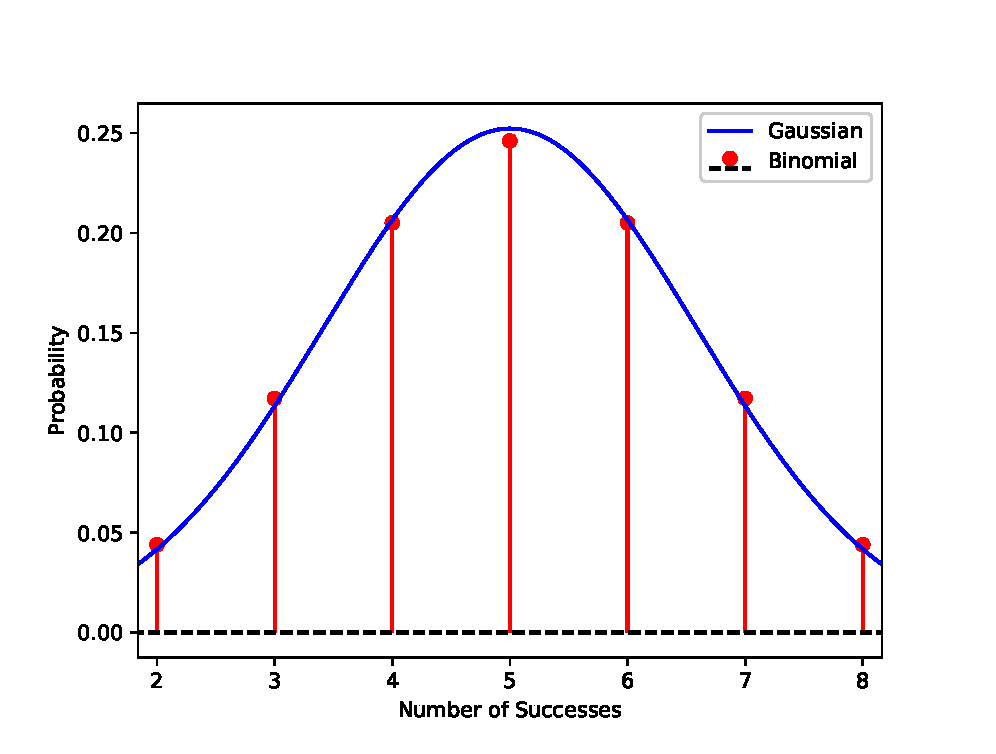
\includegraphics[width=\columnwidth]{figs/10.eps}
  \caption{10 trials}
  \label{fig:1}
\end{subfigure}
\begin{subfigure}{0.7\textwidth}
  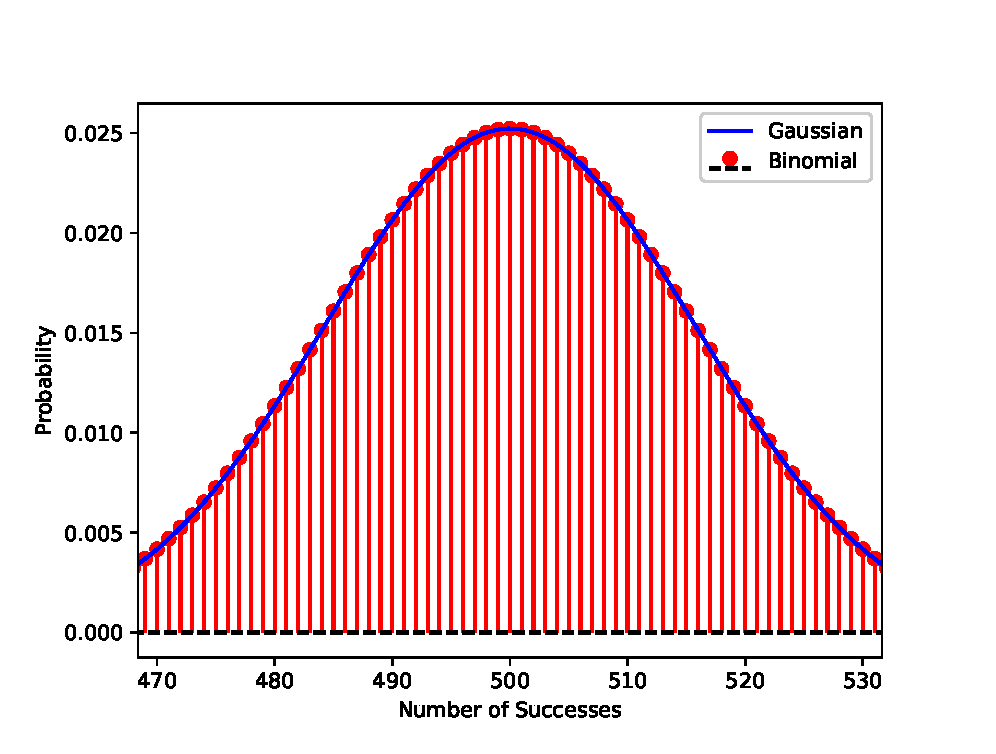
\includegraphics[width=\columnwidth]{figs/1000.eps}
  \caption{1000 trails}
  \label{fig:2}
\end{subfigure}
\centering
\caption{A comparison of Binomial and Gaussian}
\label{fig:set}
\end{figure}
\end{document}